\chapter{Background}
\label{cha:background}
This chapter provides an overview of the text mining field along with previous work in the area and all necessary background information required to understand the major tasks involved in this project. This is followed up with an overview of the different APIs provided by Twitter to work with their platform.

\section{Text Mining}
\label{sec:textmining}
The information available in the world is growing exponentially, and the majority of this information(widely estimated at roughly 80\%) is unstructured\cite{Grimes08}. This is where text mining comes in, also referred to as Knowledge Discovery from Text(KDT).
``Text mining is the process of extracting interesting information and knowledge from unstructured text''\cite{hotho-etal-ldv-2005} and its applications tend to work in two steps, first using an Information Retrieval(IR) application to narrow the search space, and then they extract significant parts of the retrieved texts\cite{Polajnar2006}. This general process usually involves structuring a source text by means of parsing and other linguistic analysis, then finding patterns in this structured data and then interpreting this output.

Text mining is fundamentally different from standard web searching in that web searches rely primarily on information that is already known. However, the goal of text mining is to discover interesting, previously unknown information\cite{Gupta_Lehal_2009}.
There is however one key issue introduced by text mining; natural language is used by humans for communication and recording information, while computers are incapable of interpreting natural language. Humans are naturally able to find linguistic patterns in text and understand the semantics of what is being said. Computers, on the other hand, face difficulties in interpreting variations in written text through spelling, colloquialism and also the general context of the text. Nonetheless, computers have what humans do not, that is, computers are much more capable of processing large datasets at very high speeds, particularly in comparison to the human being. Thus, the objective of text mining is to combine the best of these both by creating an application that can retrieve relevant documents and then apply linguistic patterns which may be rule-based, using human-defined rules, or taught by means of machine learning techniques. This project takes the rule-based approach and as such only these techniques will be discussed.

An example of the text mining process can be seen in Figure~\ref{fig:tm}.
\begin{figure}[t]
\begin{center}
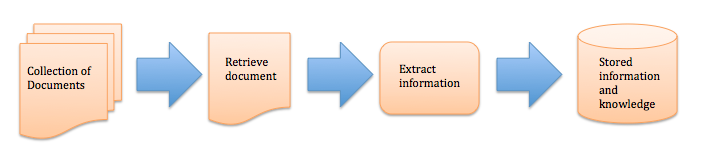
\includegraphics[width=15cm]{tm}
\end{center}
\caption{The text mining process\cite{Gupta_Lehal_2009}}
\label{fig:tm}
\end{figure}

\subsection[Information Retrieval]{Information Retrieval(IR)}
IR is the process of retrieving textual documents which may contain the answers to questions but do not answer these themselves\cite{Hearst:1999}. Information retrieval is fundamentally a web search working off user queries representing an information need. The process works by searching a collection of documents, and then retrieving those matching a user query depending on relevance. The approach to calculating relevance is dependent upon the actual IR engine itself, generally working on the frequency of specific key terms in each of these documents, and usually assigns a relevance rank to each document. This allows a sorting amongst the results and gives improved results, especially when given a limited number of results.

The IR tasks in this project will mainly be carried out on Twitter's systems, and as such, besides the core concept of IR, its internal specifics are not in the scope of this report.

\subsection[Natural Language Processing]{Natural Language Processing(NLP)}
NLP, in the scope of this project, is the process of extracting information from natural language \cite{Healey98}, that is, any language written or spoken by humans. This involves parsing and processing unstructured text to be able to gain meaningful knowledge from it. Nowadays most natural language processing is done using machine learning techniques, however, in the past implementations were based on large sets of coded `rules'. These rules are used to define certain linguistic features in the text in order to understand the semantics behind it. NLP is a major field of research at present and also has applications in both information retrieval and information extraction.

There are many methods involved in NLP tasks and some of these will now be further explored.

\subsubsection{Tokenisation}
Tokenisation is the process of splitting a stream of text into singular words or phrases, otherwise known as tokens. These tokens usually form the basis of further NLP work. While it can be a straightforward process when using Standard English, the definition of a word, from the tokeniser's point of view, can be somewhat ambiguous. This is particularly true when considering the use of apostraphes. Figure~\ref{fig:tokenisation} shows an example of the different ways of tokenising the word \emph{don't}.

\begin{figure}[h!]
  \centering
  \setlength{\unitlength}{0.0125in}
\begin{picture}(80,105)( -20, 0)
\thicklines
\put(0,100){\framebox{don't}}

\put(0,80){\framebox{dont}}

\put(0,60){\framebox{don}}
\put(30,60){\framebox{'t}}

\put(0,40){\framebox{don}}
\put(30,40){\framebox{t}}

\put(0,20){\framebox{do}}
\put(25,20){\framebox{n't}}

\put(0,0){\framebox{do}}
\put(25,0){\framebox{nt}}
\end{picture}

  \caption{The different ways of tokenising the word \emph{don't}
    \label{fig:tokenisation}}
\end{figure}

These variations can be problematic in terms of the results being output for certain user queries. For example, in the case of these differing tokenisations of \emph{don't}, a user search for the word \emph{don} would return true twice, but should be false in its actual context. The importance of normalisation is highlighted when tokenising tweets because a lot of users do not use apostrophes, either due to ease when typing, or in order to reduce the number of characters being used. Thus, varying spellings of the terms should not be tokenised differently.

\subsubsection{Normalisation}
Once text has been tokenised, these words may need normalising. Normalisation accounts for the several variations in spelling. For example, if you want to search for \emph{Mozilla~Firefox} you would want an IR engine to return not only documents containing the exact query but also those containing terms such as \emph{Firefox}, \emph{firefox} or \emph{mozilla~firefox}. Not doing this would obviously yield fewer results, or in the case of information extraction, it may suggest that \emph{Mozilla~Firefox} and \emph{mozilla~firefox} are two different things. Thus, normalisation is required to successfully map equivalent classes of terms.

\subsubsection{Stop Word Filtering}
Stop words are very commonly used words like \emph{a}, \emph{and} or \emph{the}. By creating a list of these terms, a \emph{stop list}, a natural language parser can remove these terms from the source text as they hold little or no value in matching queries to documents. In modern systems, however, stop lists are not widely used as they provide little gain in terms of efficiency\cite{manning2008}.

\subsubsection{Part of Speech(POS) Tagging}
POS tagging is a process carried out after tokenisation. Its task is to assign tags to words, for their corresponding grammatical parts of speech, based on both the word's definition, and its context. This is essentially identifying words as nouns, verbs, adjectives, etc.

However, the process is more complicated than it may first seem. The main issue is that most words do not just have one part of speech, they can have many. For example, \emph{can} could be a noun or a verb, depending on the context it is being used in. Thus, when tagging words, it is important to analyse a whole phrase or sentence. Analysing a word out of context could have significant repercussions. In the context of this project, taking the Microsoft software \emph{Paint} as an example, if someone were to tweet:
\begin{quote}
Microsoft Paint has seen some major improvements in its latest release!
\end{quote}
This would differ from, say,
\begin{quote}
Paint something now.
\end{quote}
where \emph{paint} is being used as an imperative verb. In the first example, seeing that \emph{Paint} is followed by \emph{seen}, a verb, suggests it is unlikely \emph{Paint} is being used as verb.  This would be the difference in this project between discovering a piece of software and totally missing it, and thus highlights the importance of context and semantics when analysing text.

\subsubsection{Stemming and Lemmatisation}
Documents contain many different derivations of words, such as \emph{normalise} and \emph{normalisation}, and differing forms of the same word due to its usage or tense, for example, \emph{walked} or \emph{walking}. An information extraction tool should ideally see these as somewhat equivalent terms; this is where stemming and lemmatisation come in. The following example, taken from \cite{manning2008}, shows how these techniques can map text:

\begin{quote}
am, are, is \begin{math}\Rightarrow\end{math} be 
\newline
car, cars, car's, cars' \begin{math}\Rightarrow\end{math} car
\newline
\newline
the boy's cars are different colors  \begin{math}\Rightarrow \end{math}
\newline
the boy car be differ color
\end{quote}

Stemming is a heuristic process hoping to achieve this goal by simply building basic forms of words by removing affixes like a plural `s' from nouns or the `ing' from verbs\cite{hotho-etal-ldv-2005}. However, these are not always correct terms. Lemmatisation on the other hand utilises a more sophisticated approach in that it uses a vocabulary and morphological analysis of words, in order to return to the true base form of a word that may be found in a dictionary. This process, however, is much more complex and time-consuming than the former.

\subsection[Information Extraction]{Information Extraction(IE)}
The goal of IE is to extract specific data from a given corpus\footnote{A collection of documents}. IE can be defined as the task of automatically extracting this structured information from unstructured or semi-structured machine-readable documents, generally done through the use of NLP techniques.

In structured texts, information extraction can be fairly straightforward, as labels or tags may delimit strings that need to be extracted\cite{soderland99}. However, in unstructured texts, information is not as clearly understandable by computers and so IE requires techniques from other fields such as machine learning, statistical analysis or those previously discussed from natural language processing.

Typical IE tasks include the following:

\subsubsection{Named Entity Recognition(NER)}
The aim of NER is to annotate a source text with markup tags in order to classify strings representing predefined categories such as names, companies, locations, dates and times. For example,
\begin{quote}
Cook named new Apple CEO.
\end{quote}
would yield the following annotations.
\begin{quote}
<ENAMEX TYPE="PERSON">Cook</ENAMEX> named new
\newline
<ENAMEX TYPE="ORGANIZATION">Apple</ENAMEX> CEO.
\end{quote}

This example is using the \emph{ENAMEX} tags defined at the Message Understanding Conference(MUC) in the 1990s\cite{grishman96muc}. From the source text it can be seen that \emph{Cook} has been identified as a person and \emph{Apple} as an organisation and structures this text in doing so.

\subsubsection{Relationship Extraction}
This works with entity extraction in that it works to identify relations between entities. Using the previous example, the relationship extraction process should be able to identify that,
\begin{quote}
PERSON named new ORGANISATION CEO.
\end{quote}

% OTHER SUB TASKS?

\section[Sentiment Analysis]{Sentiment Analysis and Opinion Mining}
Sentiment analysis, also known as opinion mining, refers to the NLP application of extracting subjective information in source texts. There are two use cases for sentiment analysis. The first of these is determining whether a text is subjective or objective, that is, whether the statement is factual or opinionated. This scenario is not currently in the scope of the project and leads to the second use case; sentiment analysis also aims to classify the \emph{polarity} of a given text\cite{Pang+Lee}. This, to the basic level, involves determining whether an expressed opinion is positive, negative or neutral, but can also be extended to more complex emotions such as happy or sad.

Opinion mining can be done using a weighting system. This method assigns a positive or a negative weighting on a given scale such as -3 to +3. These are applied for each word in the text that relates to the core entity. The text is then given a total score which determines its polarity, and also the strength of the sentiment. In simpler systems the scale may only be from -1 to +1, essentially opting to ignore the strength of the sentiment and just asking for the general sentiment of the text.

% More?

\section{Twitter Mining}
There has been several previous works on text mining Twitter posts, however, the bulk of these have focussed primarily on biomedicine and the financial sector. These works have shown the potential in Twitter has for providing valuable knowledge and information it is felt that software is a new area of interest where Twitter has not previously been used to analyse public opinion. Twitter's low character limit means users have to express their opinions explicitly and encourages the use of emoticons, such as :) or :(, which have been shown to work very well in sentiment analysis\cite{Read:2005}.

% MORE

%\section{Evaluation Measures}
%In text mining, there are several ways of evaluating the accuracy of a system.
%\subsection{Precision}
%\subsection{Recall}
%\subsection{F-Measure}

\section{Twitter API}
Twitter provides three public APIs for developers to access their massive corpus of data. These are the REST, Search and Streaming APIs, and shall now be further explored.

\subsection{Search API}
The Search API is the simplest tool provided by Twitter. This API is designed to allow users to query for Twitter content and works very much like the search bar found on the Twitter website itself. This content may include a set of tweets with specific keywords or tweets to, from or mentioning a specific user. A simple search would yield up to 1500 of the latest tweets in the last 7 days, which have been cached over a 60 second period. There are, however, restrictions on the rate at which programs can utilise this API\cite{twitter}.

\subsection{REST API}
The REST API enables programs to access more of the core Twitter functions. This API retrieves not only the information taken from the Search API but also allows building timelines and retrieves more specific user information such as the user's name, profile avatar, tweet count and the number of followers and friends they have. The REST API also allows programs to post on Twitter and carry out other functions like retweeting or favouriting tweets. These extra functions, however, are not required in this project.

\subsection{Streaming API}
Twitter's Streaming API is a real-time sample of all public tweets posted on the sample. It allows filtering in various ways such as user id, keywords or even random sampling, and is regarded as the default option for data mining operations. This is because the Streaming API allows a long-lived HTTP connection unlike the other APIs and as such, programs can constantly remain connected so as to retrieve a running stream of tweets, as the name itself suggests. This removes the overheads associated with reconnecting every time you want to make a query and the API also removes all rate limitations so there is no worry of exceeding your quota. Unlike the other APIs, programs must be authenticated to use the Streaming API.



